\section{Preliminaries: data representation dependent approach}\label{sec:oldschooldi}
The data integration approaches over specific data representations produced a vast amount of literature with little scientific advancement. The lack of generality forced the authors to repeat the same strategies under different possible data structures (between \textit{semistructured} XML data \cite{APoggi06}, among \textit{relational tables} \cite{Magnani09}, between \textit{structured} and \textit{semistructured}  documents \cite{ManolescuFK01,Lu2006,Magnani06}). Moreover, the lack of uniformity in these approaches led to similar results achieved at different abstraction levels (compare \cite{GolfarelliMPRT12} with the general schema alignment approach in \cite{euzenat2013d}). This latter approach proved to be interesting on the long run: it is recently used both theoretical \cite{VirgilioMT15} and more practical scenarios, such as data integration among federated data warehouses with different schemas  \cite{GolfarelliMPRT12}. 


Moreover, instead of associating an uncertainty to each schema representation and providing all the possible combinations for schema integrations \cite{Magnani09}, from the very beginning of this thesis, we’re going to consider a more flexible approach considering only the final schema to which all the data sources must comply. 

Even though we’re going to discuss the difference between structured and semistructured data in depth in Chapter \ref{cha:datadef}, we’re going to show how the approaches as mentioned above could be all generalised using the schema alignment (also known as ``ontology alignment'') approach. We refer to such chapter for additional details concerning the data representations that are here just mentioned in passing. We provide some examples on how to integrate different semistructured formats (representing graphs) into graphs (Section  \vref{sec:ngusecases}) and vice versa (Section \vref{subsec:representingisa}) in the following chapters of this thesis.








\subsection{Structured Data integration: Integrating entities represented with different schemas}\label{subsec:treunouno}
\index{data!structured} 
Given that both Data Warehouses require an associated schema towards which the data sources are transformed, and that most of the Data Warehouse literature relies on a multidimensional representation of relational databases (ROLAP), we can freely assume that Data Warehouses are structured data stores. We can now extend and adapt their use cases to the relational model, like the ones already presented in \cite{GolfarelliMPRT12}. The following example provides an use case that will also be restated for other data structures.

\begin{example}[label=ex:firstThesis]
\index{data integration!structured}
A  set of local health-care departments share some internal knowledge into a peer-to-peer Business Intelligence network. Within this network, such departments exchange medical records concerning the patients. Moreover, all such departments have different data representation for the same concepts.

Suppose that one department wants to retrieve all the records about the cured patients in both its structure and in an external department: provide a uniform representation for the patients using the local representation format.

The local data warehouse provides a table \texttt{Admissions}, as depicted in Figure \ref{tab:Admissions}: we now want to grasp all the admissions from remote locations, which may store the same entities with different relation names and with different data schemas. An example is the \texttt{Hospitalization} relation in Figure \ref{tab:Hospitalization}, where the ICD-9-CM\footnote{\url{https://web.archive.org/web/20140212190115/http://www.who.int/classifications/icd/en/}} field refers to a machine-readable representation categorizing patients' diseases.
\end{example}



After retrieving the two aforementioned tables to be integrated, the associated schemas\footnote{For both structured and semistructured data, the \textbf{schema} represents the ``patterns'' through which the data is represented using a specific data model. In this case, the tables' headers plus their associated data types represent their schema. See Chapter \ref{cha:datadef} for more complete details.} must be extracted and compared, as showed in Figure  \ref{fig:relalign}: this preliminary step is required before actually integrating the data, because we must first detect which are the fields describing the same concepts in both relations. This comparison process at the schema level is called \textbf{alignment}\index{alignment}, and it will be addressed in Section \vref{subsec:ontaling}.


We can subsume the schema alignment as follows:
\begin{alphalist}
	\item \label{lab:item:strua} each attribute having the same name will contain the same concept and, whether similar concepts are represented in different formats and representations, some transcoding function\footnote{It is represented by the \texttt{stigma} Greek letter: $\Stigma$, $\stigma$. }\index{transcoding|see{$\stigma$}} $\transcoding$ is associated \cite{GolfarelliMPRT12}. Otherwise, a correspondence is required:
	\item \label{lab:item:strub} if terms between the two schemas are similar (e.g., synonyms), they are aligned as in \ref{lab:item:strua}. Last, 
	\item \label{lab:item:struc} if there is no perfect match, then either one attribute $A$ is more general than the other $B$ ($A$ is a \textbf{supertype}\index{supertype!zzzza@\igobble |seealso {type}} for $B$  \cite{deII}, $A\sqsupseteq B$), or vice versa ($A\sqsubseteq B$); when $A\sqsupseteq B$, then the conversion is not always possible (e.g., if you have a \texttt{Week} number, you cannot map this information into a precise \texttt{Day} of the month), but the reverse process is always possible through a transcoding $\transcoding'$. Please note that all the transcodings could be either inferred using other ontologies\footnote{See Section \ref{sec:ontology} for more details.} or by using techniques exploiting artificial intelligence inference tools which suggest such relations. Therefore, the ways how such alignments may be provided are beyond the targets of the present thesis.
\end{alphalist}

\begin{example}[continues=ex:firstThesis]
 Regarding Figure \ref{fig:examplesrelational}, an ontology may detect that the \texttt{Diagnosis} allows to identify a \texttt{Disease}, and hence the two fields shall provide the same content. This scenario fits case a: since they represent a description, no translation is required; the \texttt{ICD-9-CM} code offers a \texttt{Diagnosis} for a disease and such code describes a disease: a transcoding from one concept to the other is then required.

  Last, since \texttt{Day} is part of the \texttt{Week} and since each \texttt{Month} could have several \texttt{Week}s, an ontology can infer the \texttt{Week} to which a \texttt{Day} belongs to from the information of \texttt{Day} and \texttt{Month}: this  ``alignment''\index{alignment} step must be handled as described on case \ref{lab:item:struc}.

  The final result for table \texttt{Hospitalization} to match the schema of \texttt{Admissions} is then showed in Figure \ref{tab:HospitalizationAlign}: first, we associate to each field how such alignments have to be solved (Figure \vref{fig:relalign}), and then definitively solved (Figure \ref{tab:HospitalizationTransf}) before being merged through a ``union'' in the \texttt{Admissions} table (Figure \ref{tab:MergedTables}).
\end{example}




%%%%%%%%%%%%%%%%%%%%%%%%%%%%%%%%%%%%%%
%%%%%%%%%%%%%%%%%%%%%%%%%%%%%%%%%%%%%%
%%%%%%%%%%%%%%%%%%%%%%%%%%%%%%%%%%%%%%
\subsection{Semistructured Data Integration: Integrating multiple relations into a common representation}\label{sec:SDIIMRIACR}
\index{data!semistructured}
In the previous subsection we saw one possible way of performing data integration, that is the integration of local data with external sources. Moreover, data was represented in a tabular form. Now, 
we want to integrate together \textit{(i)} different concepts \textit{(ii}) described using no explicit schema, \textit{(iii)} while representing the final data with an uniform representation. The third condition also implies that no (global) matching schema is provided. In this scenario, we require that the schema must be extracted in a (semi)automatic fashion from the data sources. As we are going to address in Section \ref{sec:datamodelling}, this is always possible because, to each datum stored in a field and using a specific data representation, we can always associate a \textbf{type}\index{type}. 
Let us now change the scenario slightly:

\begin{example}
	\index{data integration!semistructured}
  Suppose now to cope with complete medical records, which are represented in two distinct data source as semistructured XML \index{XML} documents with different associated schemas. The records shall track the patient from the admission (``Hospitalization'') to the discharge from the hospital. 
  
  Integrate such records belonging to both the remote hospital and  local hospital, while preserving the whole information coming from the two distinct sources.
  
 If we just focus on the semistructured representation provided from the data source in Figure \vref{fig:APoggiXML}, we  see that three distinct concepts are represented: the patients that entered the hospital (\texttt{<patient>\dots </patient>}), whether this patient was cured (\texttt{<treatment>\dots </treatment>}) and which ward he attended (\texttt{<ward>\dots</ward>}). On the other hand, Figure \ref{fig:ManolescuXML}  represents the patients (\texttt{<patient>\dots </patient>}) and a record associated with him/her (\texttt{<record>\dots</record>}). Given this data, we want to obtain the final result provided in Figure \vref{fig:XMLDataMergeAfterAlignment}, using an intermediate representation between the two.
\end{example}



\begin{figure}
    \begin{minipage}[t]{\textwidth}
      \lstinputlisting[language=JavaScript,basicstyle=\ttfamily\small]{fig/01dataint/xml02_apoggi_schema.json}
      \subcaption{Representng the local clinical record using the schema in \cite{APoggi06}.}
      \label{fig:APoggiSchema}
    \end{minipage}

    \begin{minipage}[t]{\textwidth}
      \lstinputlisting[language=JavaScript,basicstyle=\ttfamily\small]{fig/01dataint/xml02_manolescu_schema.json}
      \subcaption{Representing the local clinical record using the schema in \cite{ManolescuFK01}.}
      \label{fig:ManolescuSchema}
    \end{minipage}
    \caption{Representing the schema associated to the XML files using the notation provided in \cite{BaaziziLCGS17} for JSON documents. Instead of associating values to each property, we associate properties to their types. Arrays of \texttt{T} elements are represented with the \texttt{[T*]} syntax, where \texttt{T} may represent another record, representing a composite type.}
    \label{fig:XMLSchemaInJSON}
\end{figure}
\begin{figure}[!p]
	\centering
	\begin{minipage}[t]{\textwidth}
		\includegraphics{fig/01dataint/AlignmentXML02.pdf}
		\subcaption{Complete alignment process of the two schemas associated to the XML files. The green lines remark the alignments between the schemas, the blue lines mark the key detection within a local schema. When these terminological correspondences (edges) do not directly connect identical values which may appear in internal fields, such field is marked with a filled circle. The red question marks underline the fields that are missing in the other schema, and that will be filled with missing fields.}
		\label{fig:XMLAlignment}
	\end{minipage}
	\begin{minipage}[t]{\textwidth}
		\lstinputlisting[language=JavaScript,basicstyle=\ttfamily\small]{ fig/01dataint/xml02_integratedschema.json}
		\subcaption{Merged schema resulting from the hschema alignment process.}
		\label{fig:XMLSchemaMergeAfterAlignment}
	\end{minipage}
	\caption{Alignment process between the XML schema, and final XML schema integration}
\end{figure}

The data integration process seems quite hard at first because no schema is associated to the original data. 
The extraction of an associated schema  is always possible \cite{BaaziziLCGS17} and, as a result, we're going to apply the schema alignment on top of such extracted representation. Figure \vref{fig:XMLSchemaInJSON} provides the associated schema to the two XML files in a JSON format\footnote{Even though there are standard and conventional ways to associate schemas to XML files such as \textbf{XML Schema} \cite{VlistXS}, \textbf{RelaxNG} and \textbf{DTD}, and given that it is always possible to convert an XML file into JSON, I here prefer to show the XML schema using a more compact JSON representation. Both XML and JSON are, anyhow, semistructured data representations.}. At the schema level we observe that while schema (\subref{fig:APoggiSchema}) describes a person's full name through the \texttt{Surname} and \texttt{Name} tags,  schema (\subref{fig:ManolescuSchema}) only provides a \texttt{name} field. 
If we extend our schema comparison to the actual hospitalised patients’ records in both medical structures, we could then infer that name in  (\subref{fig:ManolescuSchema}) contains both \texttt{Name} and \texttt{Surname} in (\subref{fig:APoggiSchema}). Where this is not possible, we could always assume that we have a personal data bank of \textit{names} and \textit{surnames}, through which detect which part of \texttt{name} contains a name and which contains a surname. Schema (\subref{fig:ManolescuSchema}) also provides some more fields that are not in (\subref{fig:APoggiSchema}), such as the \texttt{date of birth (dob)} and the patient's \texttt{address}. By using an external ontology, we may also know that \texttt{medication} in (\subref{fig:ManolescuSchema}) corresponds to \texttt{treatment} in (\subref{fig:APoggiSchema}) and, given that the only field which has an associated  \texttt{Str}(ing) in it is \texttt{description}, then \texttt{medication} and \texttt{treatment} shall both contain the same type of content. We can also infer that \texttt{record} is a supertype\index{supertype} of \texttt{treatment} because the first contains more fields than the latter one.


\begin{figure}[!p]
	\begin{minipage}[t]{\textwidth}
		\lstinputlisting[language=XML,basicstyle=\ttfamily\small]{fig/01dataint/xml02_manolescu.xml}
		\subcaption{Representing the local clinical record using the schema in \cite{ManolescuFK01}.}
		\label{fig:ManolescuXML}
	\end{minipage}
	
	\begin{minipage}[t]{\textwidth}
		\lstinputlisting[language=XML,basicstyle=\ttfamily\small]{fig/01dataint/xml02_apoggi.xml}
		\subcaption{Representing the external clinical record using the schema in \cite{APoggi06}.}
		\label{fig:APoggiXML}
	\end{minipage}
	
	\caption{Representing two possible medical records for the same patient  coming from different hospitals.}
	\label{fig:XMLIntegration}
\end{figure}
\begin{figure}[!p]
	\lstinputlisting[language=XML,basicstyle=\ttfamily\small]{fig/01dataint/xml02_integratedata.xml}
	\caption{Expected outcome of the XML data integration. Missing values are represented by tags with no contents.}
	\label{fig:XMLDataMergeAfterAlignment}
\end{figure}
As a second step, we can make some assumptions on which fields  represent a key field within each single data source, by comparing the data in Figure \vref{fig:APoggiXML} and the associated schema in Figure \ref{fig:APoggiSchema}. We notice that \texttt{cure} is a synonym for \texttt{treatment}, and hence they can refer to the same concepts:  by comparing the  data sources,  values in \texttt{cure} correspond to values in \texttt{trId} which has a functional dependency with \texttt{treatment}. We can infer that \texttt{admitted} refers to a \texttt{SSN} because they have the same type; if more sophisticated tools are available (e.g., ontologies) by knowing that an \texttt{hospital} can \texttt{admit} a \texttt{patient},  we can also infer that \texttt{SSN} is a key for \texttt{patient}, which contains the \texttt{SSN} field, and that \texttt{admitted} refers to a \texttt{patient}. This assumption could also be confirmed by looking at data values.





Figure \ref{fig:XMLAlignment} provides all the matches inferred for the schema  alignment process, including the previous steps described in words. This alignment also allows to extend the ``syntactic'' semistructured schema integration approach presented in  \cite{BaaziziLCGS17}, and it consequently provides the merged schema depicted in Figure \ref{fig:XMLSchemaMergeAfterAlignment}. At this point, we can transform both sources  to match the provided schema using transcoding functions, and then provide a global representation of such integrated data as already presented in Figure \vref{fig:XMLDataMergeAfterAlignment}. As the last step, we could integrate all the fields that pertain to the same entity using clustering techniques (in this case, we can merge all the patients having the same SSN id). Section \ref{sec:indatabase} addresses this last part while focusing on dimensionality reduction and data cleaning processing. Moreover, if the use ontologies which are powerful enough to express that ``\textit{an Italian SSN contains information concerning the date of birth of a person}'', then such information could be easily imputed using some associated transcoding functions.

By comparing the alignments \index{alignment} process for structured data and the one for semistructured data, we observe that the schema alignment process is  data representation independent, and that all the computational steps reduce to a comparison of either fields (in the relational case) or compound fields (in the semistructured one) defining \textit{entities}\index{entity}, which appear in two different schemas. After the former comparisons, correspondences are found.
Section \vref{sec:ngusecases}  is going to further investigate this topic,  where we're going to answer the following question: ``\textit{is it possible to express both schemas and alignments within the same representation?}''.

\begin{figure}
  \lstinputlisting[language=XML,basicstyle=\ttfamily\small]{fig/01dataint/xmlrel03_integratedata.xml}
  \caption{Merging the two relational tables from Subsection \ref{subsec:treunouno} with the XML document resulting from Subsection
  	\ref{sec:SDIIMRIACR}. This data integration step  fills in the missing values marked with {\color{red}\textbf{?}}. After analysing the schema alignments paired with the to-be-aligned data, we can draw more guesses than the ones initially formulated for providing Figure \vref{fig:XMLDataMergeAfterAlignment}.}
  \label{fig:XMLDataMergeWithTheTwoTables}
\end{figure}

%%%%%%%%%%%%%%%%%%%%%%%%%%%%%%%
%%%%%%%%%%%%%%%%%%%%%%%%%%%%%%%
%%%%%%%%%%%%%%%%%%%%%%%%%%%%%%%
%%%%%%%%%%%%%%%%%%%%%%%%%%%%%%%
\subsection{Structured and Semistructured data integration: schema alignment as a data cleaning step}\label{subsec:datacleaningintegrate}
\index{data integration!structured}\index{data integration!semistructured}
\index{data cleaning}
\index{alignment}
Given the considerations of the former paragraph, we would like to use the outcomes of the data integration process presented in Section \ref{subsec:treunouno} as imputations for 
the missing values coming from the semistructured  integration phase. In particular, we want that such data can be integrated with the \texttt{ward} and the \texttt{ICD-9-CM} pieces of information coming from the \texttt{Hospitalization} table.
We must now use both the source data (Figure \vref{tab:Admissions}) and the transcoding functions generated from the alignment between the two schemas (Figure \vref{fig:relalign}). Firstly, we still have to create correspondences between each XML \texttt{treatment\_entry} and a record belonging to either \texttt{Admissions} or \texttt{Hospitalization}. 
As previously noticed, it is not possible to retrieve the precise day of the week of the \texttt{Admission} of a patient if no further precise information is known: for this reason, we're going to use the following transcoding\index{transcoding} function\iffalse for presenting the data in the extended XML format \fi, where the day information is coded through a day null value, $00$:
\begin{equation*}
\transcoding^{-1}(week,month,year)=\textup{``}00/month/year\textup{''}
\end{equation*}
Concerning the data coming from the external sources, we can still associate  a \texttt{ICD-9-CM} code to each \texttt{disease} representing a \texttt{diagnosis} through the  $\transcoding'$ given above.

Figure \ref{fig:XMLDataMergeWithTheTwoTables} provides the outcome of this alignment and integration phase: as we can see, the data imputation phase required for data cleaning may resemble the data integration steps (see Section \ref{sec:indatabase}). The only missing pieces of information are the patient's address (that could be easily retrieved after another data cleaning process after which the \texttt{patient} record will be merged), and the symptoms related to the ``Right vestibular deficit''. 

If no symptoms are provided, we can now ask ourselves if it still possible to retrieve this information from full-text medical books: which is the best way to represent such information in order to answer the question ``\textit{Which are the symptoms for balance disorders?}''?



%%%%%%%%%%%%%%%%%%%%%%%%%%%%%%%
%%%%%%%%%%%%%%%%%%%%%%%%%%%%%%%
%%%%%%%%%%%%%%%%%%%%%%%%%%%%%%%
%%%%%%%%%%%%%%%%%%%%%%%%%%%%%%%
\subsection{Integrating unstructured data via semistructured representation}\label{sec:idifud}
\index{data integration!unstructured}
Unstructured data represents digital information that cannot be immediately used as pieces of information until its transformation in a semantic dependent form is provided \cite{OrgKno}. Unstructured data usually has no associated description for interpreting such information. Figure \ref{fig:unstructuredmedical} provides some examples of unstructured contents: the index at bottom left represents an association between some medical terms represented in a hierarchical form and some ICD-9-CM codes, while the picture represents a tumour of the salivary glans. As we will see in Section \vref{sec:unstructured}, full-text content shall be represented either in a purely syntactical structured form (\textit{spans}), or in a semistructured representation. Such representations include graphs (\textit{universal dependencies graph})\index{graph!dependency graph} and nested graphs\index{graph!nested graph}\footnote{Since both nested graph data integration is proposed for the first time by this thesis, we refer to Section \vref{sss:ngdi} for further details.} (proposed by this thesis in Section \vref{sec:semistructunstradata}). Suppose now that we want to integrate the three textual representations altogether: we cannot mix them at the textual level because full-text documents could be represented in different formats (txt, doc, RDF, wiki markup or pdf) and may also express different concepts requiring different interpretations. As a consequence, the best way to integrate unstructured data is to first provide them  some structure reflecting their semantics, and  then try to merge the data.
\begin{figure}
	\centering
	\includegraphics[scale=0.7]{fig/01dataint/foldedfulltext}
	\caption{Different possible types of unstructured information: full-text sentences from Wikipedia (top left), alphabetical indices (top right), taxonomy indices (bottom left) and pictures (bottom right).}
	\label{fig:unstructuredmedical}
\end{figure}

\begin{figure}
	\centering
	\begin{minipage}[t]{\textwidth}
		\centering
		\includegraphics[scale=.8]{fig/01dataint/04_fromfulltext01.pdf}
		\subcaption{Representation of the alphabetical index in a graph form.}
		\label{fig:alphaasgraph}
	\end{minipage}
	\begin{minipage}[t]{\textwidth}
		\centering
		\includegraphics[scale=.8]{fig/01dataint/04_fromfulltext02.pdf}
		\subcaption{Representation of the taxonomy as a graph, where the association between the ICD-9-CM codes is explicit.}
		\label{fig:astaxonomy}
	\end{minipage}
	
	
	\begin{minipage}[t]{\textwidth}
		\includegraphics[width=\textwidth]{fig/01dataint/04_fromfulltext03.pdf}
		\subcaption{Integration of the two indices as a common graph, thus representing an ontology.}
		\label{fig:astaxonomy2}
	\end{minipage}
	\caption{Representing full-text contents as graphs.}
	\label{fig:mergedgraphsfromfull}
\end{figure}
\begin{example}
We now want to merge the two indices presented in Figure \ref{fig:unstructuredmedical} to create an ontology allowing the detection of clusters of similar diseases\footnote{\url{https://github.com/jackbergus/DISeASE}}. We cannot directly combine the two indices into one single file, because each file must be processed differently; while the taxonomy is a tree where all the terms point to the most general term, the alphabetical index is a graph where each general term shall point to the most specific sub-item. In the last scenario, each of these terms are disambiguation terms and directly depend on the main synset. In the previous indexing structure, distinct terms could be related to the same concept represented by a unique ICD-9-CM code: e.g., both ``vestibular vertigo'' and ``peripheral vertigo'' lead to the same concept, labelled as 386.10, classified within the taxonomy as ``Peripheral vertigo, unspecified'' (not showed).
  
  As a consequence, different graph representation techniques shall be adopted for distinct files: Figure \ref{fig:mergedgraphsfromfull} represents an example of how such indices could be first represented (\subref{fig:alphaasgraph} and \subref{fig:astaxonomy}), and then merged into one single graph (\subref{fig:astaxonomy2}), thus providing an ontology. The integration of the two graphs is merely performed via a union of the vertex and edge set.
\end{example}


\begin{figure}
\hspace*{-2cm}
  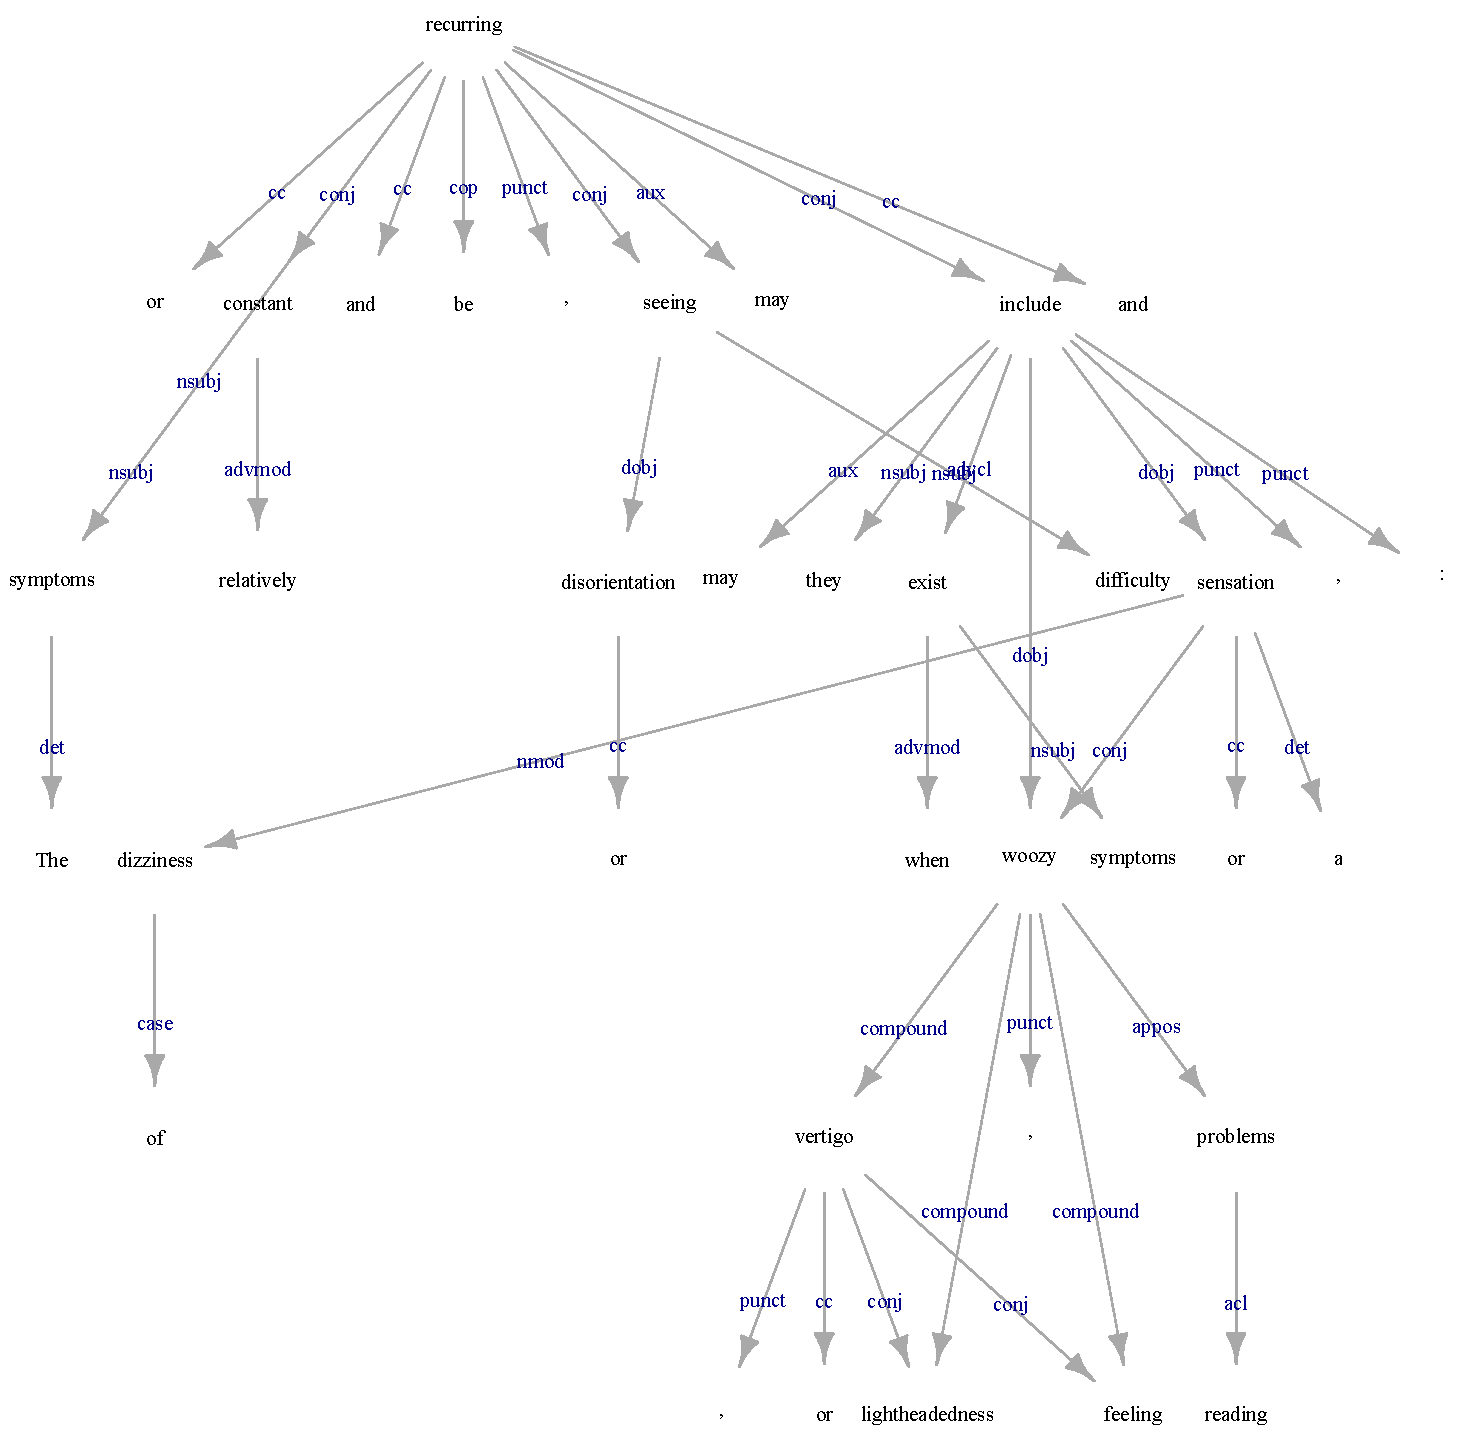
\includegraphics[width=1.3\textwidth]{fig/01dataint/recurringgrapj.pdf}
  \caption{Dependency graph of the wikipedia fulltext in Figure \ref{fig:unstructuredmedical} obtained via the Stanford NLP Library (See my source code at \url{https://bitbucket.org/unibogb/sherlock/src}). Each vertex represents one word within the full-text document, while each edge expresses a part of speech grammatical function, called \textit{universal dependency} (\url{http://universaldependencies.org}) \cite{MarneffeDSHGNM14}, which may also be (human) language dependant (i.e., different languages may provide a different set of language dependencies).}
  \label{fig:dependencygraphexample}
\end{figure}

The graph representations provided in the last example are not the sole one possible for full-text corpora: Figure \ref{fig:dependencygraphexample} provides an example of the NLP interpretation of the top left full-text from Figure \ref{fig:unstructuredmedical}, that is also machine-readable. Section \vref{sec:unstructured} is going to present more insights concerning the need for an intermediate representation of unstructured data.

\subsection{Aligning (Nested) Graphs}\label{sss:ngdi}
\index{graph!nested graph}
If we shift the schema alignment process from (semi)structured data to graphs, it is also possible to extend the schema alignment techniques to graph schema alignments. Given that graphs are a specific case of semistructured data (because they have no strict associated schema), it is also possible to represent full-text as both data, schema and queries. Graph schema alignments are the result of the query answering process: in this scenario, we align the actual data vertices and edges instead of the data schema, and where vertices may represent variables to be instantiated for solving the desired query.

\begin{example}\label{ex:nestalign}
Let us leave the healthcare data integration scenario. Suppose that we want to answer the following question: ``In May 1898 Portugal celebrate the 400$^{th}$ anniversary of the arrival of \textbf{this explorer} in India'' \cite{IBMWatson}, where \textbf{this explorer} is the subject that has to be found, and hence the ``variable'' to be instantiated. Since this is a very general question, we have to use some full-text corpora, like the one from Wikipedia. From this full-text sources, we can extract different sentences from different pages. At this step, we want to check which part of the text matches with our question. To do this we have to first provide a nested graph representation of both the question (Figure \vref{fig:question1}) and for the two candidate answers (\subref{fig:answer1} and \subref{fig:answer2}). As we can see, nested graphs allow to nest whole concepts, such as ``the arrival of this explorer in India''  as one single vertex, thus allowing to draw an edge between the ``400th anniversary'' and this other object.
	
Even in this case, each graphs' node has neither an associated schema -- that changes from question to question -- nor a type associated to each vertex and edge. Nevertheless, we can first provide some types to the question: we have that \texttt{Portugal} is a \arialify{Place}  as well as \texttt{India}, and \texttt{explorer} is elected as a type itself since it is not a simple term of the graph. The last one also represents the goal of our question. All the verbs and nouns expressing motions are marked as \arialify{Action} (e.g., \texttt{celebrated} and \texttt{arrival}), while more generic terms are associated to \arialify{Concept}, such as Anniversary. Temporal pieces of information can be marked with a \arialify{Time} type. Before starting the alignment process, we must ask ourselves which elements are considered as \texttt{explorers} or at least \arialify{Person}s in the two candidate answers. After using an ontology such as \textbf{DBpedia}, we know that \texttt{Vasco da Gama} is for sure an explorer but, using the open world assumption, we cannot say that \texttt{Gary} is not for sure an explorer, and so we associate to him a \arialify{Person} type. In the next phase, we want to associate the place \arialify{Place} \texttt{India} to all the other geographical pieces of information within the candidate answers: while \texttt{India} perfectly matches as both type and content in the first candidate answer, we find \texttt{Kappad Beach} in the second answer. Even in this case, after using DBpedia we can infer that \texttt{Kappad Beach} is  a \textbf{part-of}\index{part of} \texttt{India}, and hence in both cases we have a perfect match. At this stage, we can also try to find the matches between the temporal vertices: while the first candidate answer has no temporal information, the first one has an information that, on the other hand, is very hard to match with the one contained in the question. At this step, we could think to provide the original question some refinements: if we have the availability of an ontology matching the concept of \texttt{400th anniversary} to a function: \[anniversary(number,when)=when-number\] then we can infer that if at time $when$ we celebrated the $number$ anniversary, then the concept shall refer to a fact occurred on the year ``$when-number$''. In this case, we will obtain $1898-400=1498$, and so we can extend the nested vertex within the question with a \texttt{when} edge and the resolved time, \texttt{May 1498}: finally, we have mined a further correspondence between the temporal aspect.
	

\begin{figure}[!p]
	\begin{minipage}[t]{\textwidth}
		\includegraphics[scale=0.8]{fig/01dataint/introduction_examples_01_answer}
		\subcaption{Candidate Answer 1: ``In May, Gary arrived in India after he celebrated his anniversary in Portugal''}
		\label{fig:answer1}
	\end{minipage}
	\begin{minipage}[t]{\textwidth}
		\includegraphics[scale=0.8]{fig/01dataint/introduction_examples_00_question}
		\subcaption{Question: ``In May 1898 Portugal celebrate the 400$^{th}$ anniversary of the arrival of \textbf{this explorer} in India''}
		\label{fig:question1}
	\end{minipage}
	\begin{minipage}[t]{\textwidth}
		\includegraphics[scale=0.8]{fig/01dataint/introduction_examples_02_answer}
		\subcaption{Candidate Answer 2: ``On the 27$^{th}$ of May 1498, Vasco da Gama landed in Kappad Beach.''}
		\label{fig:answer2}
	\end{minipage}
	\caption{Representing the question (\subref{fig:question1}) and two possible candidate answers (\subref{fig:answer1} and \subref{fig:answer2}) using nested graphs. Candidate answer 2 is correct.}
	\label{fig:firstnested}
\end{figure}
	After finding all the correspondences between the vertices and nested vertices, we have to map the \arialify{Action} entities either to edges (since edges in this graph could also represent verbs) or other entities: in this case we have that the type information is not enough because it is too general, and hence we require some term similarity, that can be even in this case achieved using term ontologies such as \textbf{Babelnet}. At this stage, we can make correspondences between the terms \texttt{landed}, \texttt{arrival} and \texttt{arrived}, and hence the \texttt{arrival} matching with \texttt{arrived} could be transformed into a verb, and hence into an edge. 
	Moreover, the result of the alignment process including such graph transformations is presented in Figure \ref{fig:aligninggraphs}. We can now finally perform some approximated graph matching techniques \cite{VirgilioMT15,Aligon201520}, after which we can observe that the second candidate answer contans all the information we are looking for and, since \texttt{this explorer} and \texttt{Vasco da Gama} match and have the same type, we can say that \texttt{Vasgo da Gama} is the answer we were looking for from the very beginning.
\end{example}

This last example showed that alignment techniques could  be used not only for aligning schemas, but also for finding correspondences within ambiguous data representations. As a consequence, this example shows that graphs could be used to represent both schemas and data, and hence could be used to represent two different and distinct concepts. Consequently, we need a language expressing graph schemas, thus generalizing the schema language for semistructured documents in \cite{BaaziziLCGS17}. Moreover, it has been also showed that graphs could also represent query languages for graphs \cite{consens1990a,GraphLogAggr,n3,Goertzel2014}: as we will se in the next section, \textsc{Data}, \textsc{Model} and \textsc{(Query) Language} represent three distinct levels within usual modelling languages, while graphs allow to collapse into one single representation.

Last, pictures can be also represented as (semi)structured data: object categorization techniques \cite{Galleguillos10} such as region-based segmentations \cite{NIPS2009_3766} can be applied to extract interesting features from the pictures. By doing so each picture is automatically associated to the features that it contains. Within the e-Health scenario, such techniques have been applied to tumour detection and classification \cite{Rouh15,Rouhi16}, where the benign forms are separated from the malignant ones. Each fragment allowing such categorization could be then stored alongside with the classification's outcome, thus providing a way to transform unstructured data to structured pictures providing informations. Moreover, pictures could be represented as hypergraphs \cite{Bretto2005} and hence also as nested graphs.

\begin{sidewaysfigure}[!p]
	\centering
	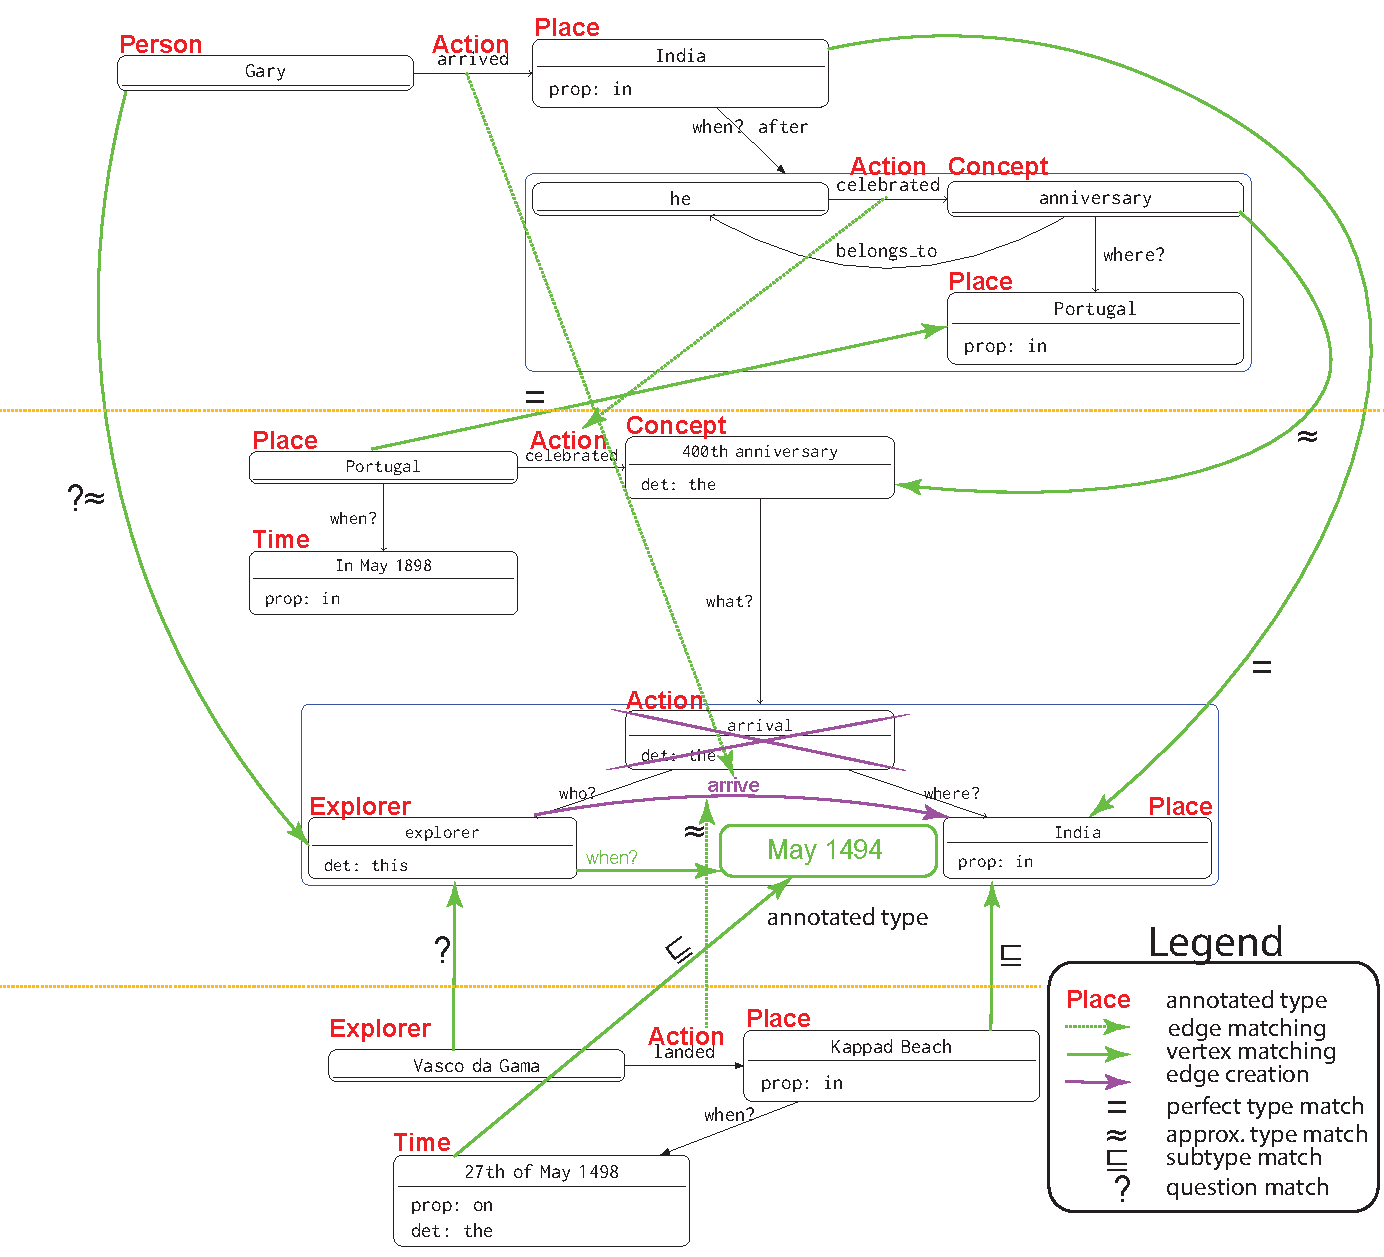
\includegraphics[width=.8\textheight]{fig/01dataint/GraphAlignWatson.pdf}
	\caption{Aligning the query to the candidate answers through nested graphs.}
	\label{fig:aligninggraphs}
\end{sidewaysfigure}

We can finally observe that, prior to allowing the integration of graphs with structured and unstructured data, we need to find a common representation for all the provided datasets. Hence, we have to discuss which is the best and general data representation allowing to represent both nested component and edges, and why such features are important and relevant. For this reason, I refer to Chapter \vref{cha:datadef} and \vref{cha:graphsdef}. Moreover, a more general approach considering data at different nesting levels is going to be discussed in Section \vref{sec:squatcases} after describing our proposed nested graph data model.

